%!TEX root = ../Thesis.tex
% Chapter Template

\chapter{Design \& development} % Main chapter title

\label{DesignDevelopment} % Change X to a consecutive number; for referencing this chapter elsewhere, use \ref{ChapterX}

\lhead{Chapter \ref{DesignDevelopment}. \emph{Design \& Development}} % Change X to a consecutive number; this is for the header on each page - perhaps a shortened title

%----------------------------------------------------------------------------------------
%	SECTION 1
%----------------------------------------------------------------------------------------

This chapter on the design and development of the algorithm will briefly touch on the development of the algorithm. The chapter will go into some detail about the design of the algorithm so that the reader may better understand the code and how the algorithms works. This chapter will also be of benefit to those who wish to use the algorithm or even modify it.

\section{Stages of development}
The thesis builds on a project proposal written by @supervisor. The proposal suggests that work be done to optimize the parameters used in the \STC algorithm in order to get better clustering results. The \CTC algorithm written by \supervisor is implemented in Python. In the project draft outlining this thesis work as preperation for the thesis, the project proposal was shifted to include the use of a genetic algorithm. This necessitated some modification of the implementation provided by \supervisor. The code is entirely written in Python 3 and provides easy ways in which to run specific parameter sets, incremental optimization, and a distributed genetic algorithm for optimization.

% I had no familiarity with Python. The \emph{first stage} of development was thus to learn Python and familiarize myself with the implementation of the \CTC algorithm. The algorithm was implemented with largely hard coded parameters with about one separate python module (file) for each parameter configuration. To make testing different parameter sets easier a \emph{second stage} of development was performed. The parameter set were abstracted away so that the clustering function would accept any parameter set. This made it possible to perform initial incremental tests. These incremental tests then informed the design of the genetic algorithm, the \emph{third stage} of development. The genetic algorithm was initially developed to run on a single computer and was designed following the specifications in \cite{Goldberg1989,Negnevitsky2002,Haupt2004a}. Testing of the initial design for the genetic algorithm revealed that it was indeed capable of improving the F-Measure of the \CTC algorithm's results. There were a problem however as testing many chromosomes on a single machine took too much time. It was necessary to distribute the task.

% A \emph{fourth stage} of development was executed to alleviate the problem. A small server - client framework was written to facilitate distribution of computation tasks. The genetic algorithm was then rewritten to send chromosomes (essentially parameter sets) to clients that would then perform the actual clustering tasks. This made it very simple to run the clustering job on multiple CPU cores and multiple computers. Additionally a corpus processor was implemented to convert other corpus files to the snippet format used for the \CTC algorithm. A new subclass of the corpus processor needs to be implemented for each additional corpus to be converted.

% \subsection{Memory handling}
% One problem with Python 2 is the way it handles memory. The client processes would, at least in some environments, consistently eat up as much memory as they could and never free up memory used. This seemed to be a problem related to the way in which Python 2 allocates and deallocates memory for small variables such as integers. Essentially the Python 2 virtual machine would hold on to memory space allocated to small variables in case it could need such space later. This in essence saves CPU cycles as it does not have to ask for more space later. The problem seemed to be that it did not reuse that space later, but instead opted to ask for a new virtual memory space for small variables. Because of this the entire project had to be ported to Python 3.

\section{Deterministic and nondeterministic behaviour}
Porting the \CTC algorithm to Python 3 proved an issue as it made the algorithm nondeterministic. The original \CTC implementation had produced consistent results. When ported to Python 3 the implementation produced slightly varying results even though the implementation was more or less the same. It turns out that the problem lied within the compact trie. In Python 2 the order in which items (key-value pairs) are inserted into a dictionary is stored implicitly. When you iterate through the items in the dictionary, they are extracted in the same order as they were inserted. This is not true for the Python 3 implementation of dictionaries. In Python 3 you are given a view when you ask for an iterator over the items in the dictionary, and this view does not return items in the same order as they are inserted. The solution was to implement the compact trie subtree maps as OrderedDictionary objects to get the same order each time. This ensure that the resulting base clusters are the same on each run of the algorithm and thus secure the consistency of the clustering results.

\section{Overview of system}
This section will give an overview of the algorithms. It will cover the overall design of the algorithms and diverge briefly into some technical aspects. The entire code base of the project is too big to be covered in its entirety. The code is open source and can be found in full at \href{http://github.com/snorremd/distributed-clustering}{GitHub - http://github.com/snorremd/distributed-clustering}. The code is licensed under the MIT license and can be used and modified freely.

\subsection{\CTC}
The original implementation of the \CTC algorithm is authored by \supervisor. The implementation used in this thesis work is more or less the same, but with modifications to allow dynamically specifying parameter sets. The \CTC algorithm is implemented as a class. The class initializer (similar to a constructor) takes as parameters a corpus object, that specifies which corpus is to be used, and a cluster settings object that informs the \CTC object if it is to include singleton ground truth clusters and which value to use for the f-beta-constant for the f-measure. Ground truth clusters are those clusters that only have a single document in it. Including those clusters may make the genetic algorithm favor solutions with many singleton clusters. The f-beta-value determines the relative weight distribution between the precision and recall values used to calculate the f-measure score. Using a very low value for the f-beta score will essentially make the f-measure a measure of precision. Conversely using a very high score will make it a measure of recall. A f-beta value of 1 makes it a harmonious mean of the two. The value can thus be used to tune the kind of results the genetic algorithm optimized for.

The initializer continues by building an index of ground truth clusters, a tag-index, and indexes over different frequency measures (corpus frequency, raw frequency and document frequency) for the terms contained within the corpus. The raw frequency of a term is the number of times that term occurs in the corpus. The ground truth index and tag index are both created based on the snippet file specified in the corpus object. The snippet file is marked up in XML and use the structure shown in Listing~\ref{lst:snippetfile}. Essentially the snippet file encompass an entire corpus. It is divided into snippet elements which correspond to one document. Each snippet is then divided into text type elements which comprise one of six forms of text from that document. Each text type element, for example ``ArticleText'', then holds snip (the actual snippets) elements that are of that text type. Finding ground truth clusters are then the simple task of finding those documents that have equal tags-values. The tag index is an index of sources (documents) pointing to the tag value of that document. It is built by collecting the source and tags-values of each document.

\begin{lstlisting}[float=ht, language=xml, breaklines=true, label=lst:snippetfile, caption={Snippet file encoded in XML}]
<?xml version='1.0' encoding='ascii'?>
<snippetcollection source="klimaukenOBT.xml">
    <snippet id="2009-12-07-aa-01" source="http://www.adressa.no/nyheter/trondheim/article1419658.ece" tags="Innenriks-ulykker-trafikk-utforkj&#248;ring-trondheim">
        <ArticleIntroduction>
            <snip> bil havne bokstavelig tale hel kant Nedre Elvehavn mandag ettermiddag</snip>
        </ArticleIntroduction>
        <ArticleText>
            <snip> bil havne hel kant Nedre Elvehavn mandag ettermiddag</snip>
            <snip> bil tom</snip>
            <snip> If&#248;lge politi S&#248;r-Tr&#248;ndealg skulle bil tom komme sted</snip>
            <snip> menneske bil politi komme</snip>
            <snip> brannvesen sikre bil Falck rekvirere berging fortelle Curt Ivar R&#248;hmen operasjonsleder S&#248;r-Tr&#248;ndelag politidistrikt</snip>
            <snip> st&#229; fri</snip>
            <snip> If&#248;lge Tr&#248;ndelag redningstjeneste skulle bil begynne rulle h&#229;nd</snip>
            <snip> forst&#229; bil st&#229; fri begynne trille stoppe kant</snip>
            <snip> sikre bil Falck berge fortelle Trond Reitan vaktleder 110-sentral</snip>
            <snip> bileier dukke</snip><snip> bare telefon bil vei elv si Tore Lagesen</snip>
            <snip> Han parkere meter kaikant overbevise bil st&#229; h&#229;ndbrekk</snip>
            <snip> n&#229; skulle bare sette godstol slappe si bileier hvilepuls</snip>
        </ArticleText>
        <ArticleByline>
            <snip> Tore Lagesen helle bil nesten ende vann Nedre Elvehavn</snip>
        </ArticleByline>
        <ArticleHeading>
            <snip> Biltur hel kant</snip>
        </ArticleHeading>
        <FrontPageIntroduction>
            <snip> En bileier Trondheim flaks side bil ta tur h&#229;nd mandag ettermiddag</snip>
            <snip> le mye</snip>
        </FrontPageIntroduction>
        <FrontPageHeading>
            <snip> telefon bil tur elv</snip>
        </FrontPageHeading>
    </snippet>
    <snippet>
      ...
    </snippet>
    ...
  </snippetcollection>
\end{lstlisting}

The \CTC algorithm is implemented as a method named clustering in the \CTC class. The application applies a chromosome, which essentially act as a parameter set (see Listing~\ref{lst:chromosome}, to the method and then executes each step of the \CTC algorithm according to the parameter values supplied. The method takes the following parameters:
\begin{inparaenum}[\itshape 1\upshape)]
\item tree type;
\item top base clusters amount;
\item min term occurrence in collection;
\item max term ratio in collection;
\item min limit for base cluster score
\item max limit for base cluster score
\item descending order
\item should drop singleton base clusters
\item should drop one word clusters
\item text types
\item text amount; and
\item similarity measure
\end{inparaenum}.

\begin{lstlisting}[float=ht, language=python, label=lst:chromosome, caption={An example chromosome}]
fitness = 0
id = 1
idCounter = 2
results = ## Ommitted
tree_type = (0,0,0)
top_base_clusters_amount = 992
min_term_occurence_in_collection = 23
max_term_ratio_in_collection = 0.72
min_limit_for_base_cluster_score = 3
max_limit_for_base_cluster_score = 7
should_drop_singleton_base_clusters= 0
should_drop_one_word_clusters = 1
text_amount = 0.73
text_types = {
  "FrontpageIntroduction": 1,
  "FrontpageHeading": 0,
  "ArticleHeading": 1,
  "ArticleByline": 1,
  "ArticleIntroduction": 0,
  "ArticleText": 1
}
similarity_measure = {
  similarity_method: 2,
  params: (0.5, 10, 1)
}
descending_order: 1
\end{lstlisting}

\subsubsection{Snippet filtering}
The first step in the \CTC algorithm is snippet filtering. The algorithm filters the snippet list according to which text types should be included. Because the parameter is randomized there are cases where the chromosome specifies that no text types should be included. In such cases the algorithm will return an empty result. An empty result is a result were each performance measure is given a zero score. The chromosome also specify a ratio that tells the algorithm how much of the article text to include. This ratio is in the range 0 \dots 1 with a .01 increment. In the event that article text should be included the number of snippets to include are then simply calculated by multiplying the number of article text snippets with the ratio.

\subsubsection{Snippet expansion}
The algorithm then moves on to the snippet expansion phase. It selects the expansion technique given by the tree type parameter in the chromosome. It may be one of the following: suffix, n-slice, mid-slice or range-slice expansion. Here the word slice is used in place of gram. Each expansion technique will be explained with an example. Given a snippet \(S\): ``mouse run trough house order find cheese is discovered cat chase away'', we can define the snippet as \(S = t_{1} \dots t_{12}\). \(S\) can be expanded using each of the four expansion techniques described below.

Each suffix phrase \(P\)  of \(S\) are defined as: \(P = t_{12-m+1} \dots t_{12}\) where \(0 \le m < 12\). This gives us the following suffixes for the snippet:
\begin{inparaenum}[\itshape 1\upshape)]
\item ``mouse run through house order find cheese is discovered cat chase away,''
\item ``run through house order find cheese is discovered cat chase away,''
\item ``through house order find cheese is discovered cat chase away,''
\item ``house order find cheese is discovered cat chase away,''
\item ...
\item ``chase away, and''
\item ``way''
\end{inparaenum}


An n-slice phrase \(P\) for slice length \(l\) is defined as \(P = t_{m} \dots t_{m+l}\) where \(0 \le m \le 12 - l\). This definition gives us the following 6-slices of the snippet:
\begin{inparaenum}[\itshape 1\upshape)]
\item ``mouse run through house order find,''
\item ``run through house order find cheese,''
\item ``through house order find cheese is,''
\item ..., and
\item ``cheese is discovered cat chase away''
\end{inparaenum}

Mid-slices are n-slices where the length \(l\) of the slices is given by the function \(l = round(\frac{phraselength}{2})\). For the example snippet the mid-slices would simply be 6-slices as exemplified above. The last type of expansion is range slices. Range slices are simply put all the n-slices in the range \(r_{min} \dots r_{max}\). Min is calculated using the function \(min = floor(snippet length * min~ratio)\). Max is calculated using a similar function: \(max = ceil(snippet length * max~ratio)\).  Min and max ratio are values where \(0 < ratio <= 1\). The range slices of the example snippet given the range 0.4 and 0.8 would thus be all n-slices in the range \(4 \dots 10\), i.e. 4-slices, 5-slices, ..., 9-slices, and 10-slices.

\subsubsection{Tree building}
The snippet expansion step returns a list of phrase source tuples. The algorithm then builds a compact trie over the list by inserting each pair into the trie structure. A simplified diagram of the structure can be seen in Figure~\ref{fig:compacttriedatastructure}. The trie is implemented as a tree structure where each node in the tree is a CompactTrie Node object. The edges in the compact trie are implemented as labels in the node. Thus the edge from the root node to one of the root's child nodes are the label property in that child node.

All nodes have a map (also known as a dictionary or associative array) of their child nodes. The map's keys are the first word in the edge labels which points to the child nodes. The values are the child nodes themselves. Empty subtree maps indicate that a node is a leaf node. All nodes expect the root node have a parent property which connects that node to its parent node. Each node also has a source property which contains a list of all sources that contains the edge label pointing to the node.

Five cases can arise when inserting a phrase source pair into the trie data structure:
\begin{enumerate}
  \item There are no edge labels out of root node beginning with first word in the phrase.
  \item There is an edge label (branch) out of root equal to that of the phrase
  \item There is an edge label (branch) out of root which starts with the same words as phrase, but phrase contains additional words
  \item There is an edge label (branch) out of root which starts with the same words as phrase, but the edge label (branch) contains additional words
  \item There is an edge label (branch) out of root which starts with the same words as phrase, but they end with different words
\end{enumerate}
In the first case inserting the phrase is no more difficult than inserting a new node with phrase as a label and source as its list of sources. In the second case the algorithm adds the source of the new phrase source pair to the existing branch node. In the third case the algorithm takes the additional words of the phrase and constructs a new node who's edge label is these additional words. It adds the source as the source list of the new node. It then makes that new node a child node of the existing branch node.

In the fourth case it finds the common start segment of the edge label and the phrase. It then makes a node where the edge label is set to the common start segment and the source list is set to the source in the phrase source pair. It then sets the edge label of the branch node to be the additional words from the original edge label, and makes the branch node a child node of the new node.

In the fifth case where the branch edge label and phrase ends with different words a new node is created for the common start segment. This segment is then set as child node of the root node. Then a node is created for the words in phrase that are not contained within the edge label of the branch node. The phrase rest node gets the source from the phrase source pair as its source list and is assigned as a child of the common start segment node. Then the edge label of the branch node is set to the words in the original branch edge label that are not in phrase, and the branch node assigns as child node of the common start segment node.

\begin{figure}[!ht]
  \begin{center}
    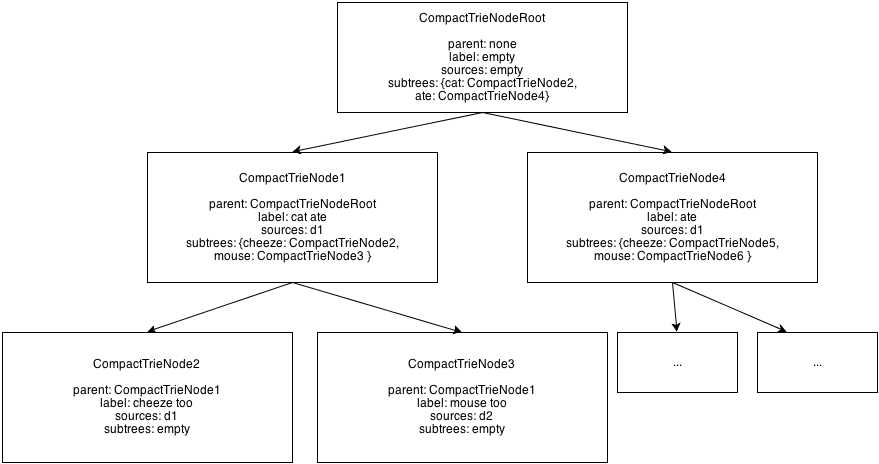
\includegraphics[totalheight=0.3\textheight]{Figures/compacttriedatastructure}
  \end{center}
  \caption{A simplified diagram of the compact trie data structure using two snippets “cat ate cheese” (d1) and “cat ate mouse too” (d2).}
  \label{fig:compacttriedatastructure}
\end{figure}

\subsubsection{Base clusters}

The \CTC algorithm generates base clusters with a simple recursive function. The function is called and applied to the root node of the compact trie. The function then creates new base clusters for each subtree in the root, and the subtrees of those subtrees etc. When all subtrees have been explored, the function iteratively adds the sources of each subtree to their parent base cluster as the function climbs out of the recursion. This way each base cluster's sources (given a node in the compact trie) is the union of all the sources in the descendant nodes.

The algorithm then sorts the base clusters according to their base cluster score. Recall the function for calculating the effective length of a base cluster label \(f(\vert P \vert)\) where \(f(\vert P \vert) = 0\) for \(\vert P \vert < 2\), \(f(\vert P \vert) = \vert P \vert\) for \(2 \le \vert P \vert < 7\), and \(f(\vert P \vert) = 7\) for \(7 < \vert P \vert\). Here the value 2 and 7 have been replaced by dynamic parameters min and max limits for base cluster scores. The min limit is a number in the range 1 \dots 5; the max limit a number in the range 3 \dots 9. If a corpus yields base clusters with generally longer labels, this will allow labels of longer lengths to be scored differently. A higher min limit will reduce the number of base clusters with short labels that might else wise be used in cluster creation.

TODO: Run analysis on base clusters produced to determine more optimal ranges.

The effective length of a label is dependent on the document frequency of each word in that label. A word contributes to a labels length if it satisfies two document frequency constraints. It should, according to \cite{Oren1998} have a document frequency of at least 4, and occur in no more than 40\% of the collection's documents. Because word frequencies vary in different corpora the optimal parameters for each of the limits might also vary. Each limit have thus been made dynamic. The first value ranges from 1 to 500, and the second from 0.1 to 1 with increments of 0.01.

\subsubsection{Base cluster merging}
Recall that \cite{Oren1998} merge base clusters using the ratio of common elements in, to the size of the union of the two base cluster sets. This implementation is fairly naive because it only considers the amount of sources the base clusters share. The implementation produces bigger clusters with good source overlap (number of shared sources), but runs the risk of producing clusters with low label overlap (few shared label words). In the research performed by \supervisor and the author of this thesis three new similarity methods have been explored. One such methods is the Jaccard Coefficient. In addition, \supervisor has experimented with coine similarity and an amendment measure which attempts to capture the similarity of the base clusters' labels.

The similarity method based on cosine similarity use the vector space model and cosine similarity function to find the similarity of base cluster labels. In this context a term's weight (tf-idf) is calculated not using it's document frequencies, but rather their base cluster frequencies. Given a base cluster \(b\), the concatenation \(S^+\) of \(b\)'s documents, and the corpus collection \(C\) the tf-idf score of a given term \(t\) in \(b\)'s label can be calculated with the function (insert cite to Richard's working paper?):

\begin{displaymath}
\vec{v}(t) = \left\{
  \begin{array}{l l}
    tf-idf(t, S^+, C) & \quad \text{if $t \in b$}\\
    0 & \quad \text{otherwise}
  \end{array} \right.
\end{displaymath}

Two base cluster labels are said to be similar if they satisfy the condition

\begin{displaymath}
\frac{\sum_{t}\vec{v}(t) * \vec{v}'(t)}
{\sqrt{\sum_{t}\vec{v}(t)^2} * \sqrt{\sum_{t}\vec{v}'(t)^2}}
\ge \theta_{cos}
\end{displaymath}

where \(\theta_{cos}\) is the threshold with which similarity is determined. A \(\theta_{cos}\) close to 1 will prevent base clusters from being merged, whilst a value close to 0 would allow close to all Jaccard similar base clusters to be merged. Finding the right \(\theta_{cos}\) should therefore be part of the optimization task.

The second similarity measure used in \supervisor working paper is one of several amendments to the Jaccard similarity measure. Under this new similarity measure two base clusters are similar if and only if they are Jaccard similar, the average corpus frequency (\(cf(w)\)) of their label words are below some threshold (\(\theta avg\)), and that they share at minimum (\(\theta min\)) number of label words. This amendment can be expressed mathematically as:

\begin{displaymath}
\frac{\sum\limits_{w \in b \cup b'} cf(w)}{\vert b \cup b' \vert} < \theta avg \quad \text{and} \quad \vert b \cap b' \vert > \theta min
\end{displaymath}

This similarity measure aims to capture those base cluster pairs who's labels indicate that the merged cluster would be extremely general. That is base cluster pairs who's average corpus frequency are higher than some threshold considered average for the collection. The measure also attempts to filter out those clusters that does not share label words.

Merging the base cluster produces a list of merged base clusters, or components. Each component is essentially a double linked list of base clusters. These components are converted to final clusters by collecting the sources and labels from the base clusters, and additionally measuring the source and label overlap of the cluster. The source overlap is the number of common sources in the base clusters in the component.

\subsubsection{Component Merge Implementation}
In the component merge step two components are merged by finding the union of the set of base clusters in the first component and the set of base clusters in the second component. There are a few ways to implement this with varying time complexities. The first implementation that was investigated uses a list implementation with a naive double for loop. For each base cluster in the second component the algorithm then loop the list of base clusters in the first component to check for the base cluster. The worst case time complexity of this algorithm is \(O(n*m)\) where \(n\) is the number of base clusters in the second component, and \(m\) the number in the first component. In some cases \(n\) and \(m\) can be almost equally big thus producing a quadratic time complexity. What this in practice means is that some parameter sets can have merge steps running for hours on end for very big base cluster amounts and low merge thresholds.

To solve this problem two additional implementations were investigated. The first attempt at a solution use simultaneous iteration over the two loops. This is done by first sorting the lists of base clusters (an at worst \(O(n \log n)\) operation). When the lists are sorted (by the base clusters' ids) one can iterate through the lists simultaneously and make sure that there is no id from component 1 that is equal to the current id from component 2. This yields a time complexity of \(O(m)\) or \(O(n)\) depending on the length of the lists. This implementation thus works very well for large values of both \(n\) and \(m\). For small values of \(n\) and large values of \(m\) it is still a good deal faster than the \(O(n*m)\) implementation, but not fast enough.

\begin{lstlisting}[float=ht, language=python, breaklines=true, label=lst:simultaneousmerge, caption={Simultaneous merge of components.}] 
base_clusters_2 = list(component2.base_clusters)
base_clusters_1 = list(component1.base_clusters)
list.sort(base_clusters_1, key=lambda bc_tuple: bc_tuple[0])
list.sort(base_clusters_2, key=lambda bc_tuple: bc_tuple[0])

i = 0  # base_clusters_1 counter
j = 0  # base_clusters_2 counter
base_clusters_add = []

while j < len(base_clusters_2):
  if i < len(base_clusters_1):
    id_1 = base_clusters_1[i][0]
    id_2 = base_clusters_2[j][0]

    if id_2 < id_1:  # This base cluster is not in base_clusters_1
      base_clusters_add.append(base_clusters_2[j])
      j += 1
    elif id_2 > id_1:  # There might be a base cluster in base_clusters_1
      i += 1
  else:  # They are the same, iterate both lists
    i += 1
    j += 1
else:  # No more base_clusters_1, add rest of two
  if id_2 != id_1:
    base_clusters_add.append(base_clusters_2[j])
    j += 1

for base_cluster in base_clusters_add:
  heappush(component1.base_clusters, base_cluster)
\end{lstlisting}
   
The second attempt at a solution use the dictionary class in Python to achieve lower time complexities. Each component implements its set of base cluster as a dictionary where the key is the base cluster's id (an integer) and the value is the base cluster object itself. The worst case time complexity of the dict object is linear time, \(O(n)\) for insert and get operations.\footnote{\href{https://wiki.python.org/moin/TimeComplexity}{TimeComplexity - Python Wiki}}. If the dict object consistently performed at worst case time complexity the run time of the algorithm would be the same as with the old list based implementation. Because the algorithm has no run time requirement for each base cluster insertion or base cluster check the worst case time complexity is not very important. Instead we can look at the average case time complexity to determine the suitability of the data structure. The average time complexity for both the insert and the get operation in the dict object is \(O(1)\), considerably better than that of default lists. The time complexity of inserting the base clusters into the component would thus be an \(O(n)\) rather than an \(O(n \log n)\) operation. The merging operation would have a guaranteed time complexity of (on average) \(O(n)\). This ensures that the merge process runs fast even for large \(m\) and small \(n\) values.

\subsubsection{Results}
Results are calculated for both the measures used by \supervisor and those used by \citeauthor{Oren1998}. See the source code for details about how the results are calculated.

\subsection{Genetic Algorithm}

\subsubsection{Genetic algorithm}
As previously written the genetic algorithm is designed to follow the specifications in \cite{Goldberg1989,Negnevitsky2002,Haupt2004a}. The genetic algorithm itself is designed as a class and has a constructor which accepts configurable settings for things like population size, mutation rate, selection rate (keep size) and selection type. Additionally it requires a database handler with which it can store results. The genetic algorithm constructor generates an initial population of the specified size.

The evolution stage have been divided into a few operations. First the algorithm calculates generational data. This includes the average fitness of the chromosomes, average numbers for the different performance measures namely: precision, recall, F-Measure, ground truth and ground truth represented. The average scores and scores held within the top, bottom and median chromosomes are all stored in a MySQL database.

After that comes the ``generation step'' which performs the evolution itself. It starts by discarding the bottom chromosomes given by the keep size. The remaining chromosomes are then used for mating. The algorithm only implements the roulette wheel selection type. Offspring are produced by slicing the parameter set in the two parent chromosomes and then combining the first and last halves respectively to form two new chromosomes.

After creating the offspring a random selection of the chromosomes in the entire population are mutated. The mutation rate and number of genes determine the number of mutations that occur in the population. The last step takes the offspring chromosomes and those chromosomes that were mutated and sends them to the task organizer which is responsible for creating execution tasks and sending them to the clustering algorithm clients.

\subsubsection{Chromosome}
The chromosome class models a chromosome in the genetic algorithm. It contains a number of genes (see Listing~\ref{lst:chromosome}) which also act as the parameter set for the \CTC algorithm. The constructor of the Chromosome class takes each parameter as a constructor parameter. The ``calc\_fitness\_score'' method applies itself as an argument to a cluster method in a ``CompactTrieClusterer'' object. In this way it sends the \CTC parameters to the clustering algorithm. The cluster method in the ``CompactTrieClusterer'' object in turn insert the clustering result into the chromosomes result property. The fitness function then use the top two F-Measure scores to calculate its own fitness. See Listing~\ref{lst:chromosomefitness} for details.

\begin{lstlisting}[float=ht, language=python, breaklines=true, label=lst:chromosomefitness, caption={Fitness function in the Chromosome class.}]
def calc_fitness_score(self, compact_trie_clusterer):
    """
    Returns the fitness of the chromosome

    Args:
        cSetting (clusterSettings): An object wrapping data
        and settings needed to run the clustering algorithm,
        the parameters in chromosome excluded.

    Calculate fitness as the average of the two
    """

    self.result = compact_trie_clusterer.cluster(self)
    fMeasure0 = self.result.f_measures[0]
    fMeasure1 = self.result.f_measures[1]
    self.fitness = fMeasure0 + fMeasure1
\end{lstlisting}

The chromosome module additionally implement a cross over function for producing offspring. This can be seen in Listing~\ref{lst:crosschromosomes}. It takes two chromosomes and retrieves their genes as tuple objects. It then crosses them by calculating a random cross over point and slicing the tuples at that position. The function then calls the ``genesTupleToChromosome'' function to create two new chromosomes for the new genes.

\begin{lstlisting}[float=ht, language=python, breaklines=true, label=lst:crosschromosomes, caption={Code for crossing chromosomes}]
def crossChromosomes(chromosome1, chromosome2):
    """
    Takes two  parent chromosomes cross them and return two children
    chromosomes
    """
    genes1 = chromosome1.genesAsTuple()
    genes2 = chromosome2.genesAsTuple()
    crossOverPoint = randint(1, len(genes1) - 1)
    genes12 = genes1[0:crossOverPoint] + genes2[crossOverPoint:len(genes2)]
    genes21 = genes2[0:crossOverPoint] + genes1[crossOverPoint:len(genes1)]

    return [genesTupleToChromosome(genes12),
            genesTupleToChromosome(genes21)]
\end{lstlisting}

\subsection{Distribution framework}
The \CTC algorithm performs rather slowly because of its \(O(n^2)\) base cluster merging step. The problem grows quadratically for n number of base clusters. Running an optimization task on the algorithm thus required that the computation of tasks were distributed. There are some great infrastructures and frameworks out there for just that kind of thing. One example is the Hadoop cluster framework which lets one implement a MapReduce task. You can then send MapReduce jobs to the main node in the Hadoop cluster and the main node will automatically find unoccupied map and reduce nodes. These frameworks were a bit too large for this thesis work, so a custom framework was implemented.

The framework consists of two parts: a server, and a client. The server handles all communication between itself, the clients and the genetic algorithm. It consists of the following main classes: Server, ClientHandler, TaskOrganizer, and a ScoreBoard. The server instance handles incoming connections and creates ClientHandler instances to communicate with the clients. Very basic authentication of clients are performed before the client is permitted to join the computation task. A client instance will send a task request message to the client handler. Upon acquisition of the message the client handler will ask the task organizer for available clustering tasks. If any tasks are available it will send these to the client handler. The client will then use a ``CompactTrieClusterer'' object to perform the clustering task and send the results back to the client handler.

The task organizer keeps a timeout index of all tasks given to a client handler. If a task has been in this index for a certain amount of time, the task will be put back into the list of available tasks. This ensures that tasks that never would have been finished, as a result of connection issues orcrashes, can be given to other clients.

Once all the tasks have been completed the task organizer sends a notify message to the genetic algorithm. The genetic algorithm then initiates its evolution method. When the genetic algorithm has finished creating a new generation of offspring, it creates new clustering tasks which is added to the list of available tasks. This cycle continues until the genetic algorithm finishes the last generation or meets a cutoff criteria. See the source code for a detailed look at how the interaction occurs.